%%%%%%%%%%%%%%%%%%%%%%%%%%%%%%%%%%%%%%%%%%%%%%%%%%%%%%%%%%%%%%%%%%%%
%% I, the copyright holder of this work, release this work into the
%% public domain. This applies worldwide. In some countries this may
%% not be legally possible; if so: I grant anyone the right to use
%% this work for any purpose, without any conditions, unless such
%% conditions are required by law.
%%%%%%%%%%%%%%%%%%%%%%%%%%%%%%%%%%%%%%%%%%%%%%%%%%%%%%%%%%%%%%%%%%%%

\documentclass{beamer}
% Compile from slides/ (editor or: latexmk -pdf -cd slides/algoritmo.tex).
% Theme sty is symlinked here; fibeamer/ and resources/ live one level up.
\usetheme[faculty=ped,basePath=../fibeamer,logo=../fibeamer/logo/mu/Logo-UC-3.png]{fibeamer}
\graphicspath{{../resources/}}

\usepackage{algorithm}
\usepackage{algpseudocode}

\usepackage[utf8]{inputenc}
\usepackage[
  main=english, %% By using `czech` or `slovak` as the main locale
                %% instead of `english`, you can typeset the
                %% presentation in either Czech or Slovak,
                %% respectively.
  czech, slovak %% The additional keys allow foreign texts to be
]{babel}        %% typeset as follows:
%%
%%   \begin{otherlanguage}{czech}   ... \end{otherlanguage}
%%   \begin{otherlanguage}{slovak}  ... \end{otherlanguage}
%%
%% These macros specify information about the presentation
\title{Algoritmos} %% that will be typeset on the
\subtitle{Semestre II-2026} %% title page.
\author{Andreina Cota Vidaurre}
%% These additional packages are used within the document:
\usepackage{ragged2e}  % `\justifying` text
\usepackage{booktabs}  % Tables
\usepackage{tabularx}
\usepackage{tikz}      % Diagrams
\usetikzlibrary{calc, shapes, backgrounds}
\usetikzlibrary{positioning,arrows.meta, shadows.blur}
\usepackage{amsmath, amssymb}
\usepackage{url}       % `\url`s
\usepackage{listings}  % Code listings
\usepackage{graphicx}
\usepackage{amsmath}
\usepackage[T1]{fontenc}
\usepackage{xcolor}
% \usepackage{adjustbox}


% Definicion de pseudocodigo en espaniol
\lstdefinelanguage{PseudocodigoES}{
    morekeywords={INICIO,FIN,PARA,HACER,SI,ENTONCES,FIN_SI,FIN_PARA,IMPRIMIR},
    sensitive=true,
    morecomment=[l]{//},
    morestring=[b]"
}

% Definicion de pseudocodigo en ingles
\lstdefinelanguage{PseudocodeEN}{
    morekeywords={BEGIN,END,FOR,DO,IF,THEN,END_IF,END_FOR,PRINT},
    sensitive=true,
    morecomment=[l]{//},
    morestring=[b]"
}

\lstset{
    basicstyle=\ttfamily\small,
    keywordstyle=\bfseries,
    columns=fullflexible,
    keepspaces=true,
    showstringspaces=false,
    frame=single,
    xleftmargin=0em,
    framexleftmargin=0em,
    framesep=2pt,
    gobble=4,
    resetmargins=true
}

\lstdefinestyle{pythonstyle}{
    language=Python,
    basicstyle=\ttfamily\small,
    keywordstyle=\bfseries,
    commentstyle=\itshape,
    stringstyle=\ttfamily,
    showstringspaces=false,
    columns=fullflexible,
    keepspaces=true,
    frame=single,
    breaklines=true,
    xleftmargin=0em,
    framexleftmargin=0em,
    framesep=2pt,
    aboveskip=0pt,
    belowskip=0pt,
    gobble=4,
    resetmargins=true,
    emph={print,input,int,float,str,bool,len,range},
    emphstyle=\bfseries
}

\lstset{style=pythonstyle}

% Estilos del diagrama
\tikzstyle{iniciofin} = [
    ellipse,
    minimum width=2.5cm,
    minimum height=1cm,
    text centered,
    draw=black,
    fill=blue!25
]

\tikzstyle{proceso} = [
    rectangle,
    rounded corners,
    minimum width=3cm,
    minimum height=1cm,
    text centered,
    draw=black,
    fill=cyan!20
]

\tikzstyle{decision} = [
    diamond,
    aspect=2,
    text centered,
    draw=black,
    fill=yellow!35
]

\tikzstyle{flecha} = [
    thick,
    ->,
    >=Stealth
]

% \newcolumntype{Y}{>{\raggedright\arraybackslash}X}

\frenchspacing
\begin{document}
  \shorthandoff{-}
  \frame[c]{\maketitle}

% \begin{darkframes}

    \begin{frame}{Contenido}
        \begin{enumerate}
            \item Algoritmo
            \item Elementos básicos del algoritmo
            \item Pseudocódigo
        \end{enumerate}
    \end{frame}

    \begin{frame}{Algoritmo}
        \justifying
        Secuencia {\color{cyan} finita} y {\color{cyan} ordenada} de instrucciones o reglas bien definidas, 
        las cuales se ejecutan en un orden específico. Es un procedimiento o fórmula paso a paso para resolver un problema.
    \end{frame}

    \begin{frame}{Algoritmo - Historia}
        \begin{itemize}
            \item Proviene del nombre del matemático persa Muhammad ibn Musa Al-Khwarizmi, quien vivió entre los siglos VIII y IX
            \item Considerado como el padre o fundador del álgebra
            \item Con el tiempo, su nombre fue latinizado y dio origen al término que hoy se conoce como {\color{cyan} algoritmo}
        \end{itemize}
        \centering
        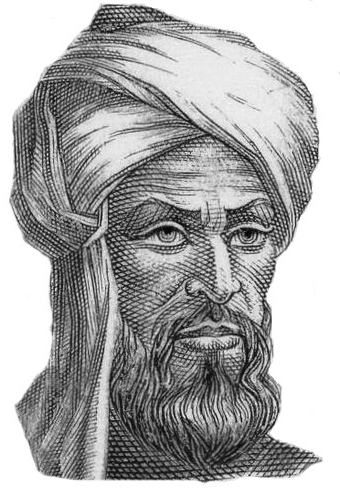
\includegraphics[width=\linewidth,height=3cm,keepaspectratio]{Al-Khwarizmi_portrait.jpg}
    \end{frame}

    \begin{frame}{Características del algoritmo}
        \begin{enumerate}%[(I)]
            \item \textbf{Finito.} Debe terminar después de un número finito de pasos
            \pause
            \item \textbf{Preciso.} Cada paso del algoritmo debe estar claramente definido
            \pause
            \item \textbf{Ordenado.} Debe seguir una secuencia lógica
            \pause
            \item \textbf{Definido.} Si se ejecuta varias veces con la misma entrada, debe producir el mismo resultado
            \pause
            \item \textbf{Con entradas y salidas.} Recibe datos y produce resultados
        \end{enumerate}
    \end{frame}

    \begin{frame}{Ejemplos del uso de algoritmos}
        \centering
        \begin{tabular}{m{0.48\textwidth} m{0.38\textwidth}}
        \onslide<1->{Preparar el desayuno} & \onslide<1->{\centering 
\includegraphics[height=2cm,keepaspectratio]{sandwich_2.png}} \tabularnewline
        \onslide<2->{Seguir la receta} & \onslide<2->{\centering
\includegraphics[height=1.5cm,keepaspectratio]{completo.png}} \tabularnewline
        \onslide<3->{Cruzar la calle} & \onslide<3->{\centering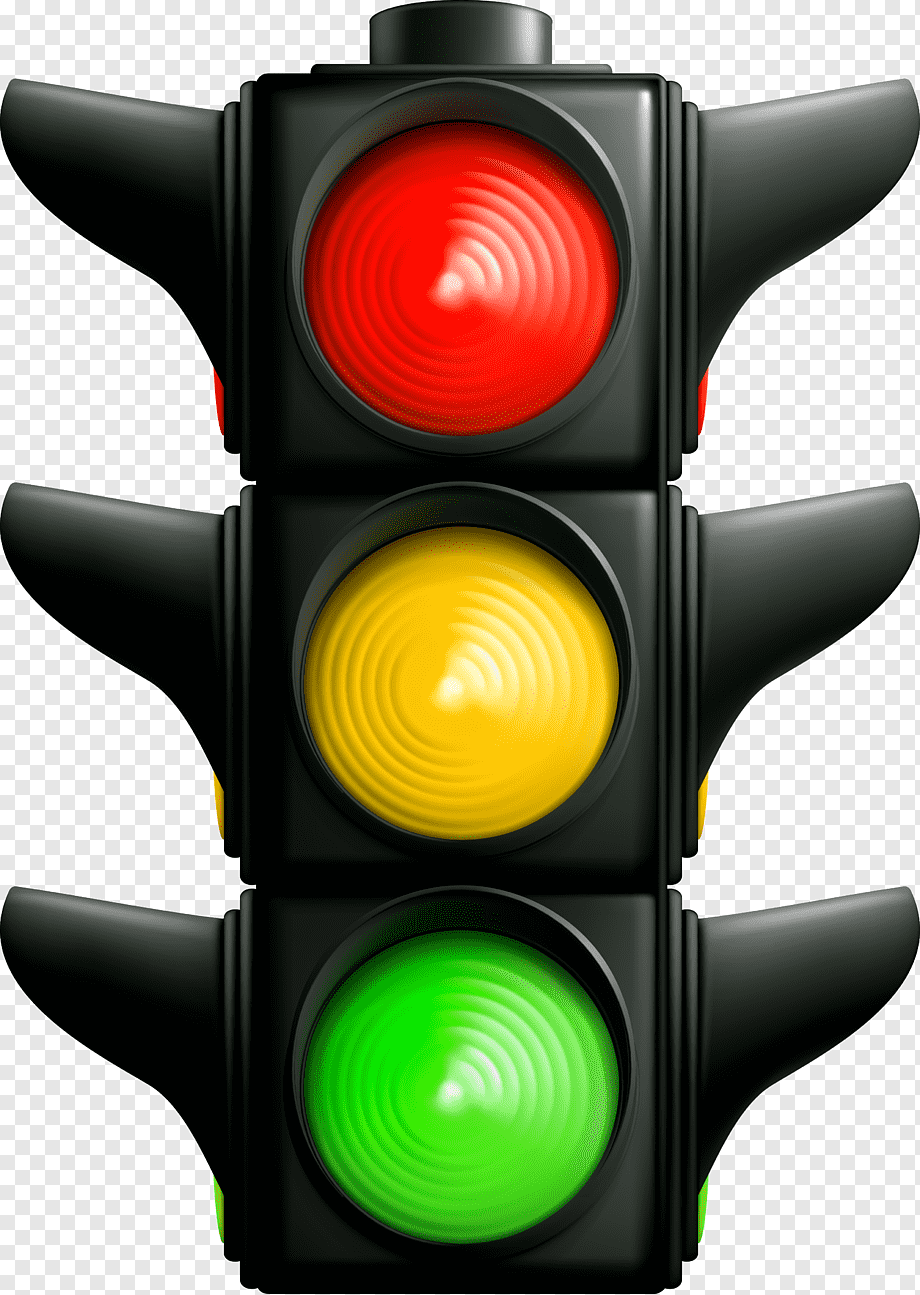
\includegraphics[height=1.5cm,keepaspectratio]{semaforo.png}} \tabularnewline
        \onslide<4->{Lavarse los dientes} & \onslide<4->{\centering
\includegraphics[height=1.5cm,keepaspectratio]{toothbrush.png}} \tabularnewline
        \end{tabular}
    \end{frame}

    \begin{frame}{¿Qué otros ejemplos podemos encontrar?}
        % \centering
        % 
\includegraphics[height=4cm,keepaspectratio]{soldado.png}
    \end{frame}

    \begin{frame}{Pseudocódigo}
        \begin{itemize}
            \item Descripción de alto nivel de un algoritmo que utiliza una combinación de lenguaje natural y estructuras de programación
            \item Permite centrarse en la lógica del algoritmo sin preocuparse por la sintaxis específica de los lenguajes de programación
        \end{itemize}
    \end{frame}

    \begin{frame}{Características del Pseudocódigo}
        \begin{itemize}
            \item \textbf{Legibilidad}. Fácilmente legible y comprensible
            \item \textbf{Simplicidad}. Se enfoca en transmitir la lógica de manera clara, sin complicaciones
            \item \textbf{Flexibilidad}. No está vinculado a la sintaxis de ningún lenguaje de programación
        \end{itemize}
    \end{frame}

    \begin{frame}[fragile]{Ejemplos de Pseudocódigo}
        \textbf{Tarea:} Sumar dos números
        % \centering
        \begin{lstlisting}[language=PseudocodigoES]
            INICIO
                LEER num1
                LEER num2
                suma = num1 + num2
                RETORNAR suma
            FIN
        \end{lstlisting}
    \end{frame}

    \begin{frame}[fragile]{Ejemplos de Pseudocódigo}
        \textbf{Tarea:} Leer tres notas y retornar el promedio
        \begin{lstlisting}[language=PseudocodigoES]
            INICIO
                LEER nota1
                LEER nota2
                LEER nota3
                promedio = (nota1 + nota2 + nota3) / 3
                RETORNAR promedio
            FIN
        \end{lstlisting}
    \end{frame}

    \begin{frame}[fragile]{Ejemplos de Pseudocódigo}
        \textbf{Tarea:} Leer un número y decir si es positivo, negativo o cero
        \begin{lstlisting}[language=PseudocodigoES]
            INICIO
                Leer num
                SI num > 0 ENTONCES
                    Escribir "Positivo"
                SINO
                    SI num < 0 ENTONCES
                        Escribir "Negativo"
                    SINO
                        Escribir "Cero"
                    FIN_SI
                FIN_SI
            FIN
        \end{lstlisting}
    \end{frame}

    \begin{frame}[fragile]{Ejemplos de Pseudocódigo}
        \textbf{Tarea:} Convertir un número binario de 4 bits a decimal
        \begin{lstlisting}[language=PseudocodigoES]
            INICIO
                LEER b3
                LEER b2
                LEER b1
                LEER b0
                decimal = b3 * 8 + b2 * 4 + b1 * 2 + b0 * 1
                RETORNAR suma
            FIN
        \end{lstlisting}
    \end{frame}

    % \begin{frame}{Ejemplos de pseudocódigo}
    %     \begin{itemize}
    %         % \item Leer un número y decir si es par o impar
    %         % \item Determinar si un número es múltiplo de otro
    %         \item Verificar si una persona es mayor o menor de edad
    %         \item Determinar si un estudiante aprobó o reprobó su nota
    %         \item Determinar si un año es bisiesto
    %         % \item Determinar si un número tiene una o dos cifras
    %         % \item Determinar si un número es capicúa de tres cifras
    %     \end{itemize}
    % \end{frame}

    \begin{frame}{Resumen}
        \begin{itemize}
            \item Algoritmo
            \begin{itemize}
                \item Es una secuencia finita y ordenada de pasos para resolver un problema 
                o realizar una tarea.
                \item Debe ser claro, preciso y sin ambigüedad.
                \item No depende de un lenguaje de programación específico, es la lógica antes del código.
            \end{itemize}
            \item Pseudocódigo
            \begin{itemize}
                \item Es una forma de escribir un algoritmo usando lenguaje natural estructurado.
                \item Sirve como un puente entre la lógica del algoritmo y el código en un lenguaje de programación específico.
            \end{itemize}
        \end{itemize}
    \end{frame}

    \begin{frame}{Material de clases}
        Mientras se habilita el acceso a la plataforma oficial, las diapositivas del curso estarán disponibles temporalmente en la siguiente carpeta: 
        \href{https://uccl0-my.sharepoint.com/:f:/g/personal/acota_uc_cl/IgBGsHN9E_Q4TZiX78b8tjXlAW5MQSzHVR0QzNv-KdNDM3M?e=pcYxmm}{Archivos de la clase}

        \begin{figure}
            \centering
            
\includegraphics[width=0.5\linewidth]{qr_intro.png}
        \end{figure}
    \end{frame}

    % \begin{frame}[fragile]{Ejemplos de Pseudocódigo}
    %     \textbf{Tarea:} Encontrar el máximo número en una lista que tiene un rango de 1 a 10
    %     \begin{lstlisting}[language=PseudocodigoES]
    %         INICIO
    %             max = primer elemento de la lista
    %             PARA cada elemento en la lista HACER
    %                 SI elemento > max ENTONCES
    %                     max = elemento
    %                 FIN_SI
    %             FIN_PARA
    %             IMPRIMIR max
    %         FIN
    %     \end{lstlisting}
    % \end{frame}

    % \begin{frame}[fragile]{Ejemplos de Pseudocódigo}
    %     \textbf{Tarea:} Convertir un número decimal entre 0 y 3 a decimal
    %     \begin{lstlisting}[language=PseudocodigoES]
    %         INICIO
    %             LEER num
    %             SI num >= 2 ENTONCES
    %                 b1 = 1
    %                 num = num - 2
    %             SI_NO
    %                 b1 = 0
    %             FIN_SI
    %             SI num >= 1 ENTONCES
    %                 b0 = 1
    %                 num = num - 1
    %             SI_NO
    %                 b0 = 0
    %             FIN_SI
    %             IMPRIMIR b3, b2, b1, b0
    %         FIN
    %     \end{lstlisting}
    % \end{frame}

    % \begin{frame}[fragile]{Ejemplos de Pseudocódigo}
    %     \begin{lstlisting}[language=PseudocodeEN]
    %         BEGIN
    %             max = primer elemento de la lista
    %             FOR cada elemento de la lista DO
    %                 IF elemento > max THEN
    %                     max = elemento
    %                 END_IF
    %             END_FOR
    %             PRINT max
    %         END
    %     \end{lstlisting}
    % \end{frame}

    % \begin{frame}{Ejemplos de pseudocódigo}
    %     \begin{lstlisting}
    %         INICIO
    %             LEER num
    %             original = num
    %             invertido = 0
            
    %             MIENTRAS num > 0 HACER
    %                 digito = num MOD 10
    %                 invertido = invertido * 10 + digito
    %                 num = num DIV 10
    %             FIN_MIENTRAS
            
    %             SI original = invertido ENTONCES
    %                 IMPRIMIR "El numero es capicua"
    %             SI_NO
    %                 IMPRIMIR "El numero no es capicua"
    %             FIN_SI
    %         FIN
    %     \end{lstlisting}
    % \end{frame}

    % \begin{frame}[fragile]{Ejemplo de pseudocódigo}
    %     Tarea: Ordenar una lista
    %     \begin{lstlisting}[language=PseudocodeEN]
    %         BEGIN
    %             REPEAT
    %                 swapped = FALSE
    %                 FOR i = 0 TO length(list) - 2 DO
    %                     IF list[i] > list[i + 1] THEN
    %                         SWAP(list[i], list[i + 1])
    %                         swapped = TRUE
    %                     ENDIF
    %                 ENDFOR
    %             UNTIL NOT swapped
    %         END
    %     \end{lstlisting}
    % \end{frame}

    % \end{darkframes}

    % \begin{frame}{Conclusión}
    %     \begin{itemize}
    %         \item El algoritmo es una secuencia de pasos ordenados y finitos que ayudan a resolver un problema
    %         \item El pseudocśodigo 
    %     \end{itemize}
    % \end{frame}

    % \begin{frame}[label=bibliography]{Bibliografía}
    %   \framesubtitle{\TeX, \LaTeX, and Beamer}
    %   \begin{thebibliography}{9}
    %     \bibitem{knuth84}
    %         Donald~E.~Knuth.
    %         \emph{The \TeX book}.
    %         Addison-Wesley, 1984.
    %     \bibitem{lamport94}
    %         Leslie~Lamport.
    %         \emph{\LaTeX : A Document Preparation System}.
    %         Addison-Wesley, 1986.
    %     \bibitem{MG94}
    %         M.~Goossens, F.~Mittelbach, and A.~Samarin.
    %         \emph{The \LaTeX\ Companion}.
    %         Addison-Wesley, 1994.
    %     \bibitem{tantau04}
    %         Till~Tantau.
    %         \emph{User's Guide to the Beamer Class Version 3.01}.
    %         Available at \url{http://latex-beamer.sourceforge.net}.
    %     \bibitem{MS05}
    %         A.~Mertz and W.~Slough.
    %         Edited by B.~Beeton and K.~Berry.
    %         \emph{Beamer by example} In TUGboat,
    %           Vol. 26, No. 1., pp. 68-73.
    %   \end{thebibliography}
    % \end{frame}

    % \subsection{Bibliografía}
    % \againframe{citations}
    % \againframe{bibliography}
\end{document}
